

\documentclass[10pt, titlepage, oneside, a4paper]{article}
\usepackage[T1]{fontenc}
\usepackage[utf8]{inputenc}
\usepackage[swedish]{babel}
\usepackage{amssymb, graphicx, fancyhdr}
\usepackage{hyperref}
\usepackage{tikz}
\usepackage{listings}
\addtolength{\textheight}{20mm}
\addtolength{\voffset}{-5mm}
\renewcommand{\sectionmark}[1]{\markleft{#1}}

\newcommand{\Section}[1]{\section{#1}\vspace{-8pt}}
\newcommand{\Subsection}[1]{\vspace{-4pt}\subsection{#1}\vspace{-8pt}}
\newcommand{\Subsubsection}[1]{\vspace{-4pt}\subsubsection{#1}\vspace{-8pt}}


\def\typeofdoc{Laborationsrapport}
\def\course{S0014D}
\def\pretitle{Laboration 5}
\def\title{Bombomanu!}
\def\name{Magnus Björk}
\def\username{magbjr-3}
\def\email{\username{}@student.ltu.se}
\def\graders{Patrik Holmlund}
\def\university{Luleå Tekniska Universitet}


\def\fullpath{\raisebox{1pt}{$\scriptstyle \sim$}\username/\path}


\begin{document}
	\begin{titlepage}
		\thispagestyle{empty}
		\begin{large}
			\begin{tabular}{@{}p{\textwidth}@{}}
				\textbf{\university \hfill \today} \\
				\textbf{\typeofdoc} \\
			\end{tabular}
		\end{large}
		\vspace{10mm}
		\begin{center}
			\LARGE{\pretitle} \\
			\huge{\textbf{\course}}\\
			\vspace{10mm}
			\LARGE{\title} \\
			\vspace{15mm}
			\begin{large}
				\begin{tabular}{ll}
					\textbf{Namn} & \name \\
					\textbf{E-mail} & \texttt{\email} \\
				\end{tabular}
			\end{large}
			\vfill
			\large{\textbf{Handledare}}\\
			\mbox{\large{\graders}}
		\end{center}
	\end{titlepage}


	\lfoot{\footnotesize{\name, \email}}
	\rfoot{\footnotesize{\today}}
	\lhead{\sc\footnotesize\title}
	\rhead{\nouppercase{\sc\footnotesize\leftmark}}
	\pagestyle{fancy}
	\renewcommand{\headrulewidth}{0.2pt}
	\renewcommand{\footrulewidth}{0.2pt}

	\pagenumbering{roman}
    \tableofcontents
	
	\newpage

	\pagenumbering{arabic}

	\setlength{\parindent}{0pt}
	\setlength{\parskip}{10pt}
	

	\section{Problemspecifikation}
		Att programmera en server samt klient som tillsammans utgör ett spel där spelare kämpar mot varandra i en kamp på liv och död. Spelet skall vara en bomberman-klon vilket innebär:
		\begin{itemize}
			\item Spelare som deltar spelar mot varandra.
			\item Spelare kan släppa ner bomber på spelplanen som exploderar efter 5 sekunder.
			\item Om en spelare blir träffad av följande explosion så förlorar denne.
			\item Siste spelare på planen vinner.
		\end{itemize}
		
		
    \section{Användarhandledning}
    	\subsection{Klient}
    		När applikationen startar möts användaren av en lista över servrar. I listans högra hörn så finns en knapp som leder till en vy där man kan lägga till fler servrar till listan. För att lägga till en server till listan måste man veta IP-adress till en server samt vilken port server lyssnar på (standardport är: 12345). För att ansluta till en server klickar man på en cell i listan.\\\\När en spelare anländer till spelplanen har denne två val:
    		\begin{itemize}
    			\item Flytta gubben genom att klicka på en position på kartan. Gubben kolliderar med andra spelare, bomber samt pelare på spelplanen.
    			\item Lägg en bomb på gubbens position genom att klicka på gubben. Efter 5 sekunder så kommer bomben att explodera. Lägger man bomber inom räckhåll för varandra så kommer den som smäller först att även detonera de bomber som finns inom räckhåll, oavsett deras interna timer. Om en spelare befinner sig inom räckhåll för explosionen så kommer denne att förlora.
    		\end{itemize}
    		
    		Spelet pågår tills dess att det bara finns en spelare kvar på planen.
    		
    	\subsection{Server}
    		En server krävs för att man skall kunna spela överhuvudtaget. Vill man ändra port från standard värde ('12345') kan man hitta detta värde i klassen ServerSocket. Trafiken är krypterad, vill man av någon anledning slå av detta så kan man göra det i klassen Socket. Där kan man även sätta vilken nyckel spelet skall använda.
    		
    	\newpage
    	
    \section{Algoritmbeskrivning}
    	\subsection{Applikationsprotokoll}
    	\subsubsection{Meddelanden}
    		Kommunikation mellan server och klient sker via ett antal meddelanden. Dessa meddelanden är structs som man sedan typecastar till char* när man skickar dem. Första post i varje meddelande är en struct MsgHead, detta gör det möjligt att behandla alla inkommande meddelanden på liknande vis genom att typecasta inkommande meddelanden till denna struct. När man sedan vet vilken typ meddelandet har kan man typecasta till korrekt meddelande typ.
    		
    	\begin{center}
    	\begin{tabular}{| l | l | l |}
    	\hline
    	\multicolumn{3}{|c|}{MsgHead}\\
    	\hline
    	Attribut & Typ & Uppgift\\ 
    	\hline
    	id & u int & Identifiering av klient. \\
    	type & enum & Avgöra hur man skall behandla meddelandet. \\
    	length & u int & Antal bytes i meddelandet. \\
    	seq\_no & u int & Ordning av meddelanden. \\
    	\hline 
    	\end{tabular} 
    	\end{center}
    	
    	Exempel på meddelande typer:
    	
    	\begin{center}
    	\begin{tabular}{| l | l | l |}
    	\hline
    	\multicolumn{3}{|c|}{EventMsg}\\
    	\hline
    	Attribut & Typ & Uppgift\\ 
    	\hline
    	head & MsgHead & Data angående meddelande.\\
    	type & enum & Vilken event-typ meddelande behandlar.\\
    	\hline 
    	\end{tabular} 
    	\end{center}

    	\begin{center}
    	\begin{tabular}{| l | l | l |}
    	\hline
    	\multicolumn{3}{|c|}{BombuMsg}\\
    	\hline
    	Attribut & Typ & Uppgift\\ 
    	\hline
    	event & EventMsg & Data angående meddelande.\\
    	pos & Coordinate & Position av bomb.\\
    	\hline 
    	\end{tabular} 
    	\end{center}
    	
    	\newpage
    	\subsubsection{Handshake}
    	Antag att klienten och servern har slutit kontakt. Nedan beskrivs hur en klient och server kommunicerar med varandra.
    	
    	\begin{center}
    		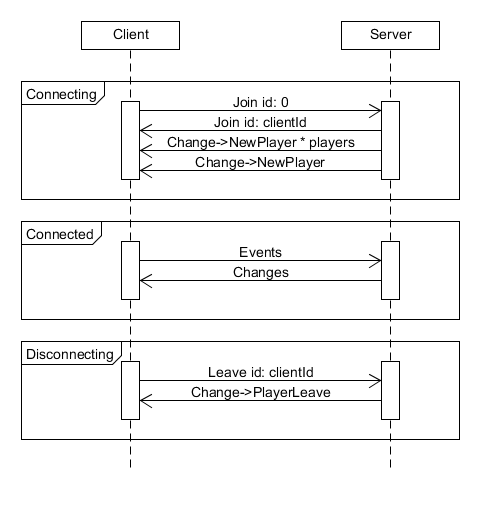
\includegraphics[scale=.5]{./png/JoinProtocol.png}
    	\end{center}
    	\begin{itemize}
    		\item\textbf{Connecting}
    		\begin{enumerate}
    			\item Client skickar Join meddelande med id == 0.
    			\item Server svarar med ett Join meddelande men har angivit ett id nummer.(id nummer är egentligen 'socket file descriptor', detta är unikt för varje ansluten klient.) Alla klientens kommande meddelanden till servern kommer att ha detta id i MsgHead.
    			\item Servern skapar nu ett NewPlayer meddelande för varje spelare som befinner sig på servern och skickar det till den nya klienten.
    			\item Servern skickar därefter den nya klienten i ett NewPlayer meddelande som går ut till alla anslutna klienter.
    		\end{enumerate}
    		
    		\item\textbf{Connected}
    		\begin{enumerate}
    			\item Klienten kan nu skicka Event meddelanden till servern.
    			\item Servern delger dessa meddelanden till alla klienter om de godkänns av modellen.(Om kollision sker under en förflyttning skulle Event exempelvis inte godkännas.)
    		\end{enumerate}
    		\item\textbf{Disconnecting}
    		\begin{enumerate}
    			\item Klient skickar ett Leave meddelande till servern.
    			\item Server delger detta till alla klienter så att dessa kan ta bort klienten från sina views.
    		\end{enumerate}
    	\end{itemize}
    	
    	\subsubsection{Förflyttning}
    	\begin{center}
    		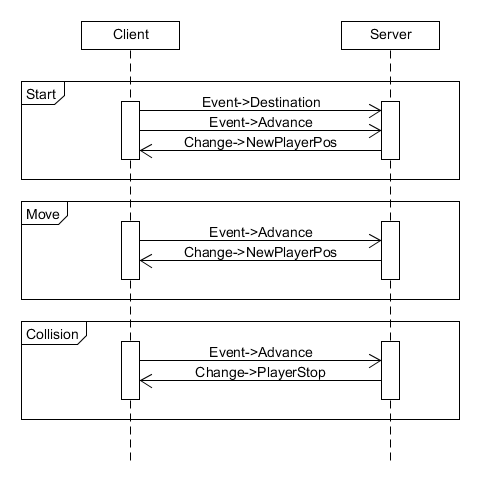
\includegraphics[scale=.5]{./png/MoveProtocol.png}
    	\end{center}
    	
    	\begin{enumerate}
    		\item När användaren trycker på skärmen och triggar en touchevent så skickas två meddelanden till servern: Event->Destination med önskad position och Event->Advance för att be om förflyttning.
    		\item När servern tar emot den nya önskade positionen registreras detta så att den kan användas i förflyttningsalgoritmen. 
    		\item När Event->Advance tas emot av servern så körs förflyttningsalgoritmen, returnerar denna sant så har spelaren förflyttat ett steg i modellen och ett Change->NewPlayerPos meddelande skickas till alla klienter(multicast). Om algoritmen returnerar falskt så betyder det att spelaren har stannat så ett Change->PlayerStop skickas tillbaka till klienten (unicast).
    	\end{enumerate}
    	
    	\newpage
    	\subsection{Path-finder}
    	Servern har en metod för att förflytta spelare, denna metod utför en algoritm för att beräkna vilken position som spelaren borde förflytta sig till. Slutdestination sätts när servertråd får meddelandet Event->Destination av klient. Därefter kommer klient att skicka Event->Advance tills dess att den får ett Change->PlayerStop från servern.
    	
    		\begin{enumerate}
    			\item Jämför spelarens position med slutdestination. 
    			\item Är markören på slutdestination? Returnera falskt.
    			\item Skapa en array av punkter. Punkterna representerar de positioner spelaren kan flytta sig i: upp, vänster, ner och höger.
    			\item Byt plats på ner<->upp och höger<->vänster beroende på hur spelarens position förhåller sig till slutdestination.
    			\item Jämför nu sträckorna i y och x-led. Prioritera den längre sträckan över den kortare. 
    			\item Gå nu igenom listan med positioner och kolla om position är giltig för förflyttning (position innehaver ej bomb eller annan spelare och är inte markerad som besökt). Om en position är giltig markera då nuvarande position som besökt och flytta markören. Returnera sant.
    			\item Är ingen position giltig för förflyttning? Returnera falskt.
    			 
    		\end{enumerate}
    	Om denna metod returnerar falskt kommer servern att skicka ett Change->PlayerStop meddelande som säger till klienten att sluta skicka Event->Advance.
    	
    	\newpage
    	\subsection{Kryptering}
    	Kryptering av trafik sker med RC4 kryptering. RC4 är ett ström chiffer som använder sig av symmetriska nycklar och består av två algoritmer:
    	\begin{itemize}
    		\item\textbf{KSA - Key-Scheduling Algorithm}\\Genererar en array [S] av chars beroende på en given nyckel.
\begin{lstlisting}[frame = single]
for i from 0 to 255
    S[i] := i
endfor
j := 0
for i from 0 to 255
    j := (j + S[i] + key[i mod keylength]) mod 256
    swap values of S[i] and S[j]
endfor
\end{lstlisting}
    		
\item\textbf{PRGA - Pseudo-Random Generation Algorithm}\\Genererar 1 char beroende av array [S] genererad med KSA. Efter att en char har genererats byter man plats på två index (i,j) i array [S] för att ytterligare slumpa arrayen.

\begin{lstlisting}[frame = single]
i := (i + 1) mod 256
j := (j + S[i]) mod 256
swap values of S[i] and S[j]
K := S[(S[i] + S[j]) mod 256]
output K
\end{lstlisting}
    		\begin{enumerate}
    			\item Börja med att skapa en array [S] av chars med värden 0 till 255.
    			\item Nu anger man en nyckel(key) och med den så kastar man om värdena i den array man skapade i punkt 1.
    			\item Man har nu en array av chars som man kan använda i PRGA för att kryptera bytes.
    			\item Har man en byte man vill kryptera så kör man helt enkelt XOR på den byten samt den byte genererad av PRGA. När man sen vill dekryptera så kör man XOR igen.
    			\begin{lstlisting}[frame = single]
   Krypterad byte = Okrypterad byte ^ K;
Dekrypterad bytee =  Krypterad byte ^ K;
    			\end{lstlisting}
    		\end{enumerate}
    		OBS: För att man skall kunna köra asynkron trafik måste man ha separata PRGA index för in och ut trafik.

\end{itemize}
    	
    \newpage
    \section{Systembeskrivning}
    	\subsection{Klient}
    		\subsubsection{ViewControllers}
    		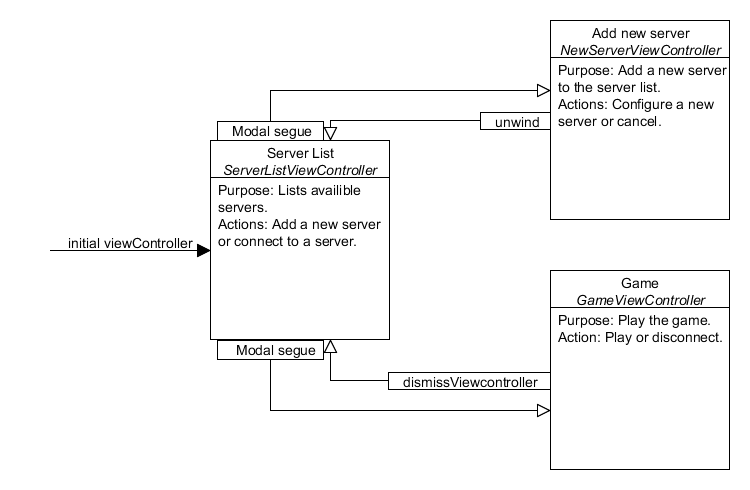
\includegraphics[scale=.4]{./png/StoryBoard.png}
    		\begin{itemize}
    			\item\textbf{NewServerViewController}
    			\item\textbf{ServerListViewController}
    			\item\textbf{GameViewController}
    		\end{itemize}
    		\subsubsection{GameScene}
    		\begin{itemize}
    			\item\textbf{GamePlayer}
    			\item\textbf{GameFinished}
    		\end{itemize}
    		\subsubsection{ThreadManager}
    		\subsubsection{Trådar}
    		\begin{itemize}
    			\item Thread
    			\item Listener : Thread
    			\item Transmitter : Thread
    		\end{itemize}
    		\subsubsection{Client: Socket}
    		
    	\subsection{Server}
    		\subsubsection{main.cpp}
    		\subsubsection{GameModel}
    		\subsubsection{Trådar}
    		\begin{itemize}
    			\item\textbf{Thread}
    			\item\textbf{BombThread}
    		\end{itemize}
    		\subsubsection{Server: Socket}
    		
   
   	

    \newpage
    \section{Diskussion}
    	\subsection{Resultat}
    	
    	\begin{enumerate}
			\item En spelare måste veta serverns URL för att kunna ansluta. När en spelare ansluter så kommer denne direkt in i ett pågående spel. Anslutna klienter är begränsade till 4-5st.i\\\textit{\textbf{Implementation:} Antalet anslutna klienter är ej begränsat, ansluter en klient så hamnar denne i ett pågående spel.}
			
			\item Spelplanen är helt blank och innehåller endast spelare. När en spelare 'tappar' på spelplanen så rör sig markören mot denna position, en annan gesture släpper en bomb på befintlig position. Står en spelare inom räckhåll för explosionen så förlorar denne. Spelet fortsätter tills dess att en spelare vunnit.\\\textit{\textbf{Implementation:} Touchevent på spelplanen flyttar spelaren, touchevent på spelaren släpper ned en bomb på spelarens position. Träffas en spelare av följande explosion så är denne ute ur spelet.}
			
			
			\item Spelplanen har hinder som spelare kan ta skydd bakom. Nu behövs även en algoritm för att markören skall flytta sig till den position spelaren 'tappade på'.\\\textit{\textbf{Implementation:} På spelplanen finns som tidigare nämnt ett antal pelare som spelaren kan ta skydd bakom. En enkel algoritm är implementerad för att förenkla förflyttningar av spelaren.}
			\\\\\textit{\textbf{Ej implementerade punkter:}}
			\item Spelplanen har sprängbara objekt som öppnar upp spelplanen för spelarna. Spelarna måste spränga sig fram till varandra.\\\textit{\textbf{Anledning:} Implementationen av hur bomberna exploderar samt sätts ut, medförde att min planerade implementation av blocken inte skulle fungera. Med tanke på tidsbrist tog jag beslutet att utesluta denna punkt och därmed även punkt 5.}
			\item Sprängbara objekt har en chans att förvandlas till en 'Power-up' som spelarna kan ta för att förbättra deras bombers egenskaper(Större explosioner, fler bomber).
			\item Animerad 2d grafik.\textit{\textbf{Anledning:}Tidsbrist.}
			\item Ljudeffekter\textit{\textbf{Anledning:}Tidsbrist.}
			\item Musik\textit{\textbf{Anledning:}Tidsbrist.}
			\item Stöd för fler spelare. Efter att (4-5) spelare har anslutit till servern så startas en ny spelplan som nya klienter kan ansluta sig till.\\\textit{\textbf{Anledning:} Applikationen körs på iOS8 och då jag endast har tillgång till en enhet (+simulator) så uteslöt jag denna punkt.}
			\item Global toplista över alla som någonsin har spelat spelet.\\\textit{\textbf{Anledning:}Tidsbrist.}
		\end{enumerate}
    	\subsection{Lösningens begränsningar}
    		\subsubsection{Klient}
    		\subsubsection{Server}
\end{document}
